%***********************************************************************
\subsection{Calibration Evaluation}\label{sub:bc_calibration_evaluation}
%***********************************************************************

% FEBA Test No. 218 Prior Uncertainty Propagation, TC
\clearpage
\begin{sidewaysfigure}
	\centering
	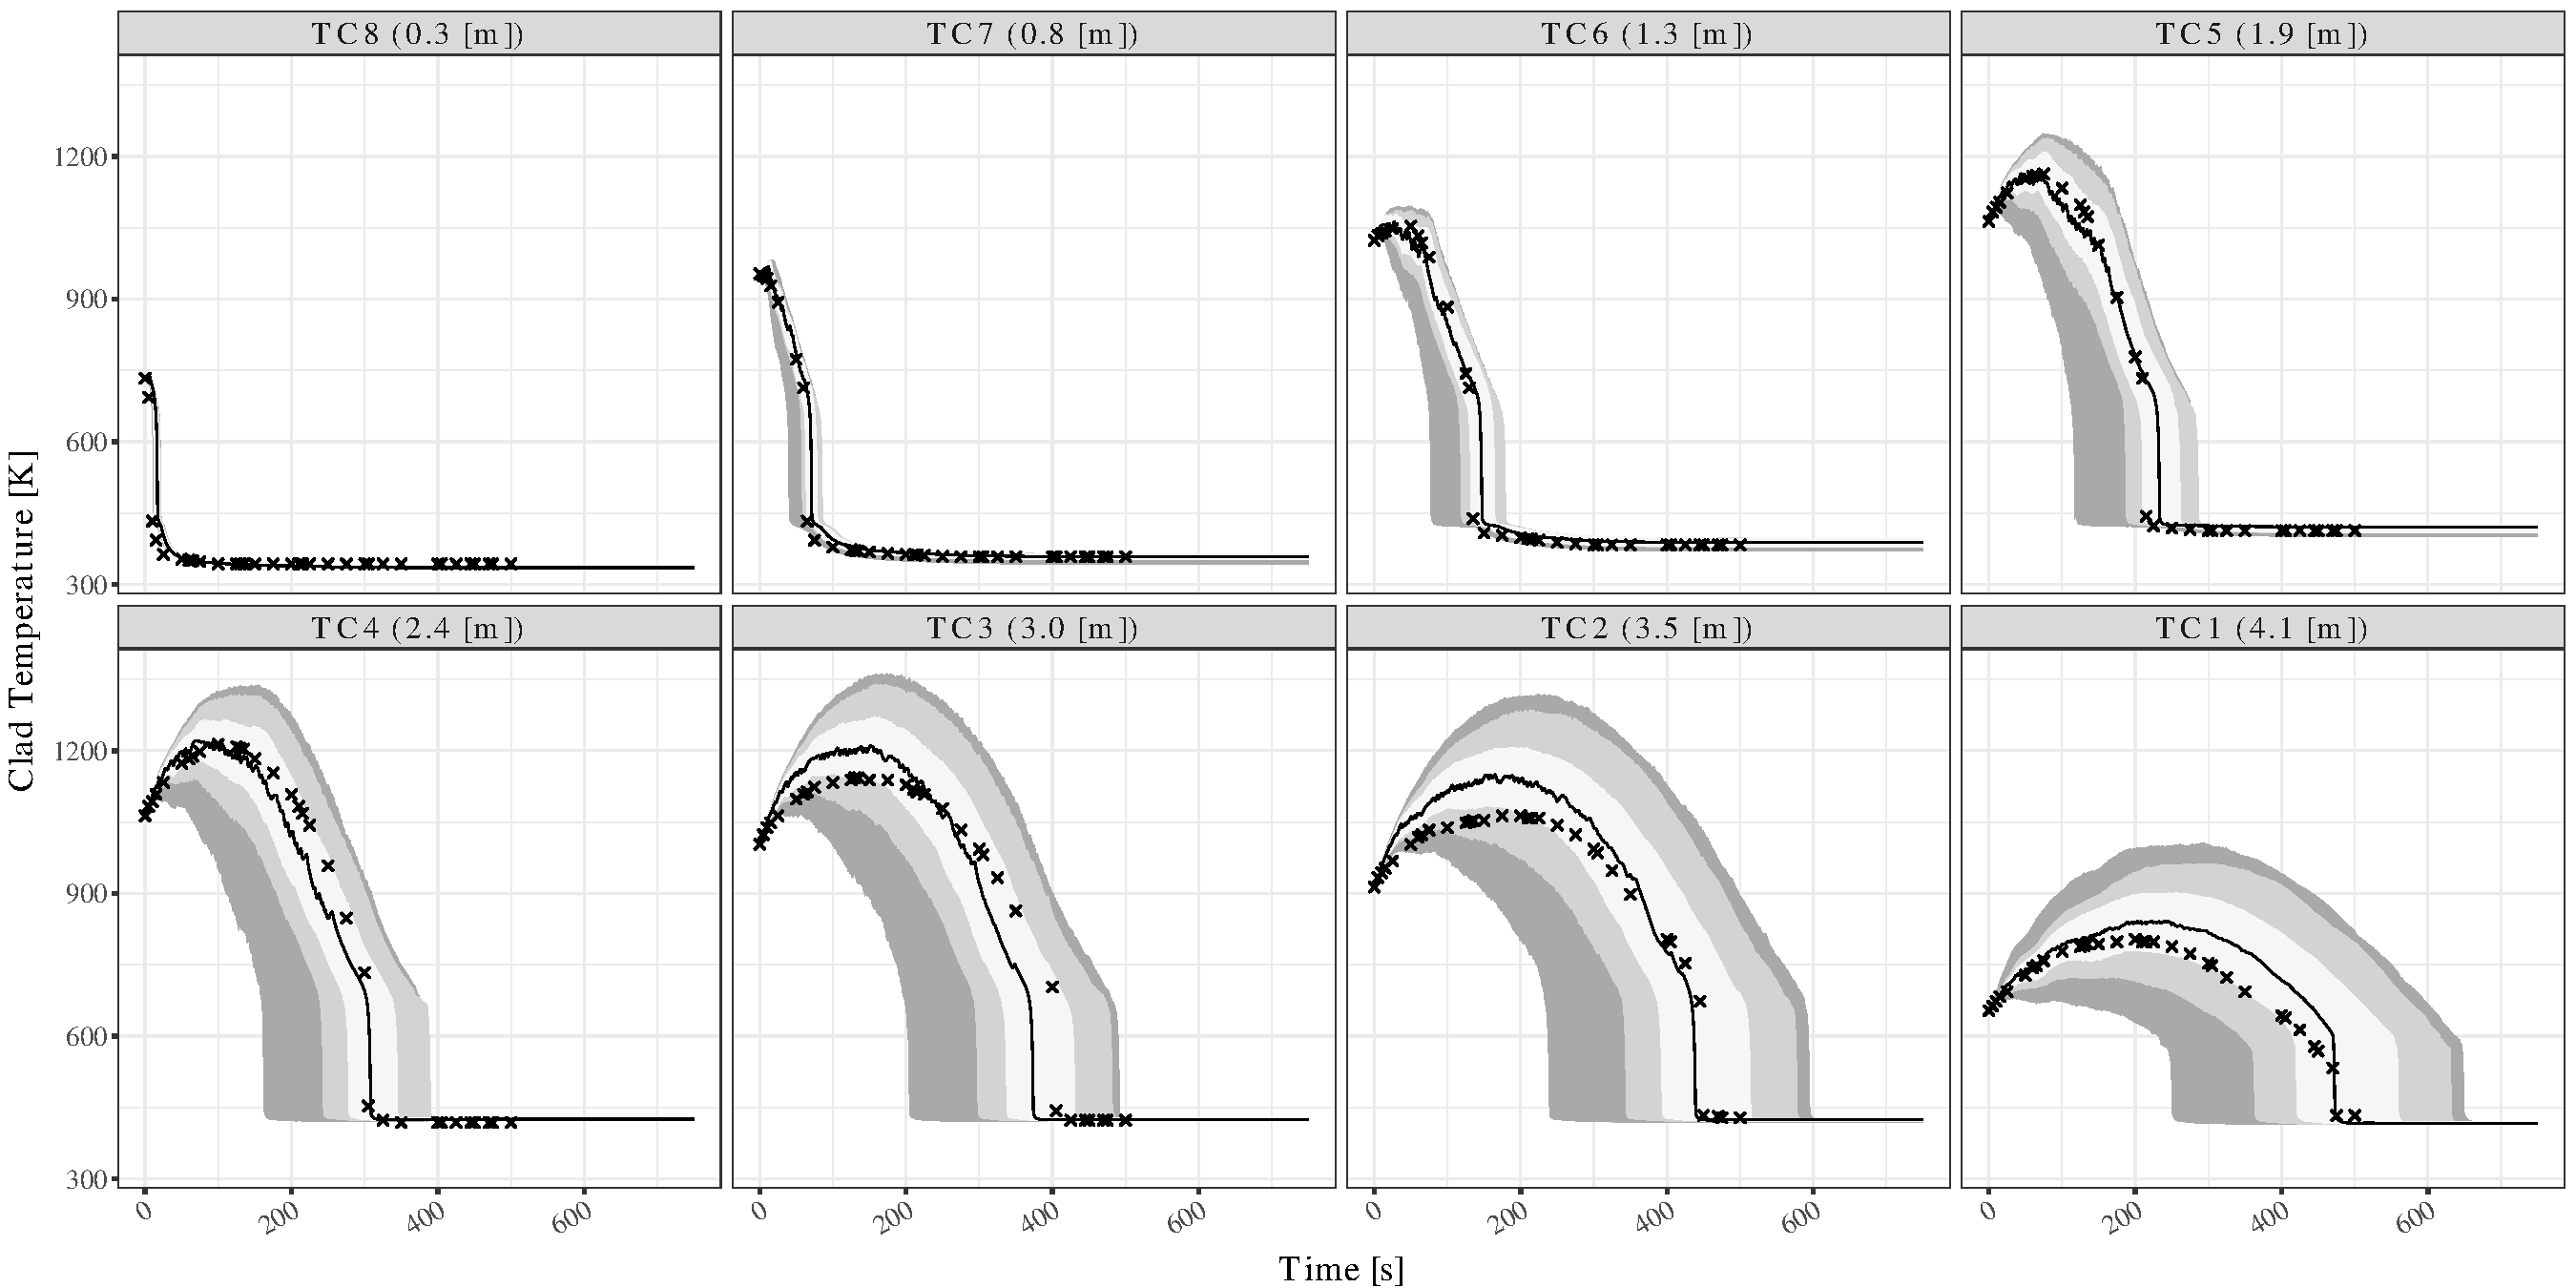
\includegraphics[width=1.0\textwidth]{../figures/chapter5/figures/plotTraceUQPosteriorAllDiscCenteredTC}
		\captionof{figure}[Calibration score vs. Informativeness for different posterior samples propagated on all the FEBA tests.]{Calibration score vs. Informativeness for different posterior samples propagated on all the gls[hyper=false]{feba} tests. Vertical lines indicate the informativeness of the prior uncertainty (defined as $0$) while the horizontal lines indicate the initial Calibration score (i.e., that of the prior).}
	\label{fig:ch5_plot_trace_uq_posterior_alldisccentered_tc}
\end{sidewaysfigure}
\clearpage

\begin{figure}[!bth]
    \centering
    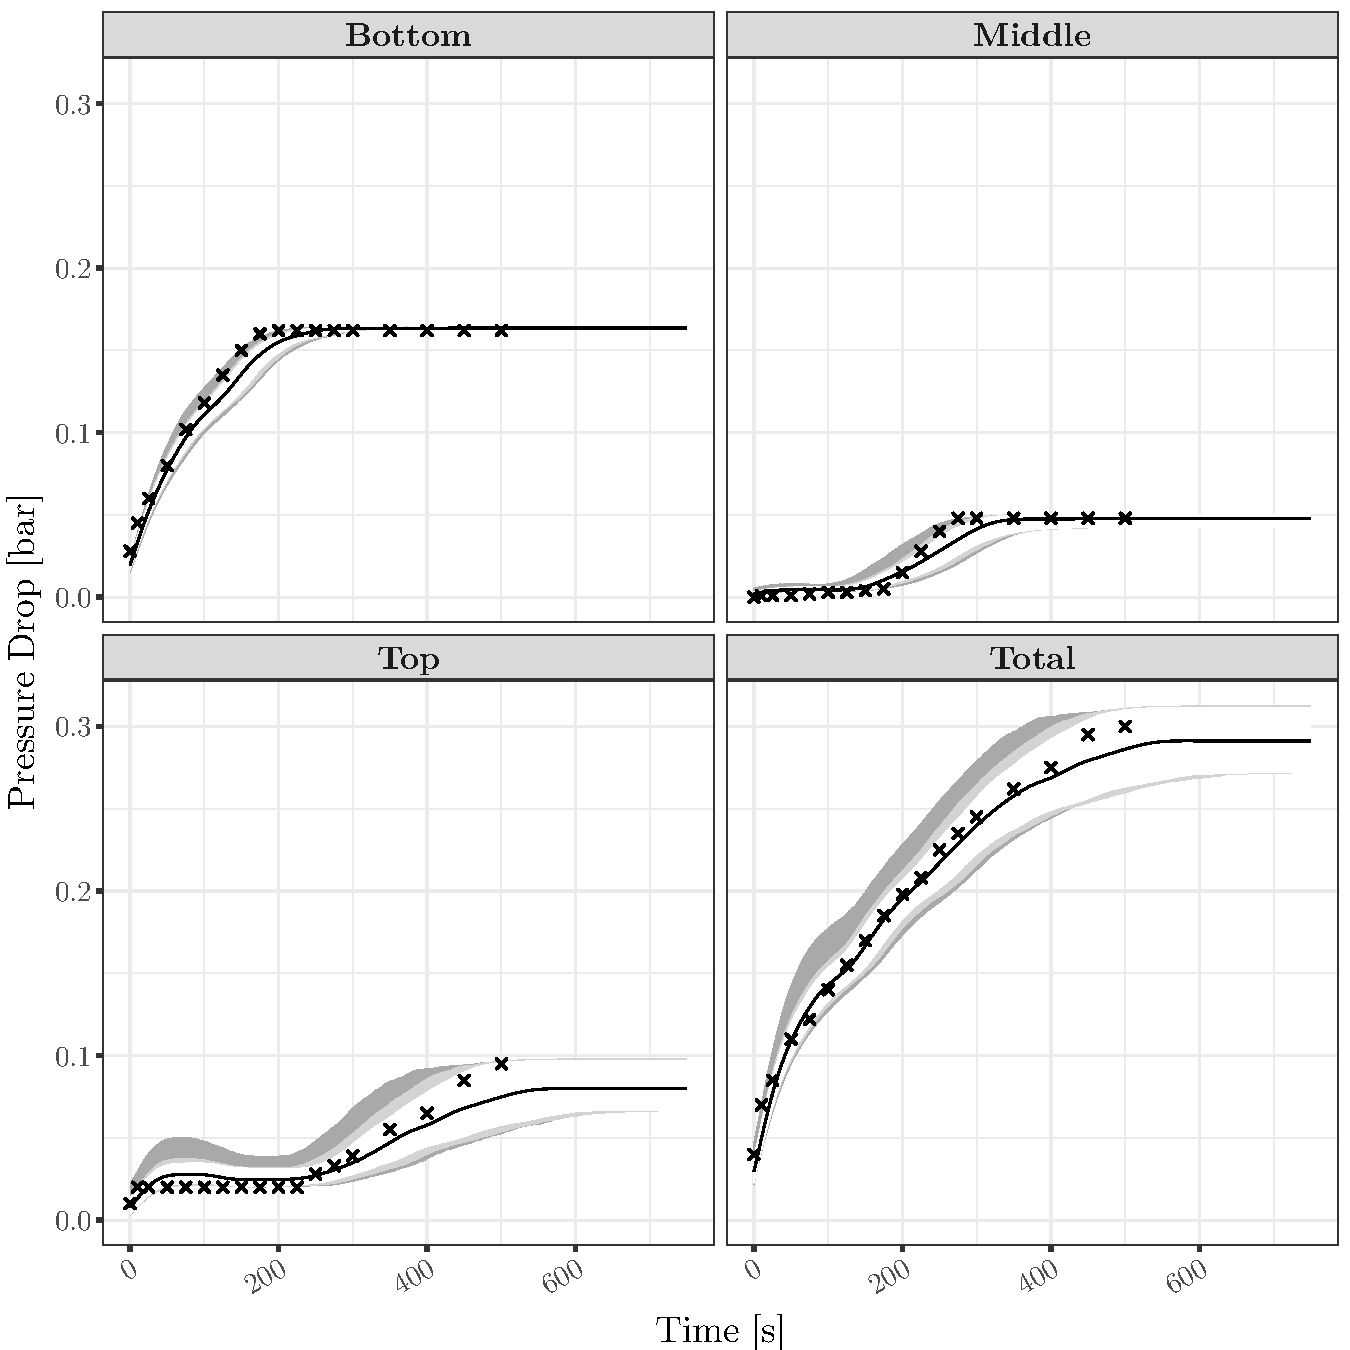
\includegraphics[width=1.0\textwidth]{../figures/chapter5/figures/plotTraceUQPosteriorAllDiscCenteredDP}
    \caption[Prior uncertainty propagation of FEBA Test No. $218$ for the pressure drop output ($DP$).]{Uncertainty propagation of the prior parameters uncertainty of \gls[hyper=false]{feba} Test No. $218$ for the pressure drop output ($TC$) at different axial segments using \gls[hyper=false]{trace}.}
    \label{fig:ch5_plot_trace_uq_posterior_alldisccentered_dp}
\end{figure}
Balaba
\begin{figure}[!bth]
    \centering
    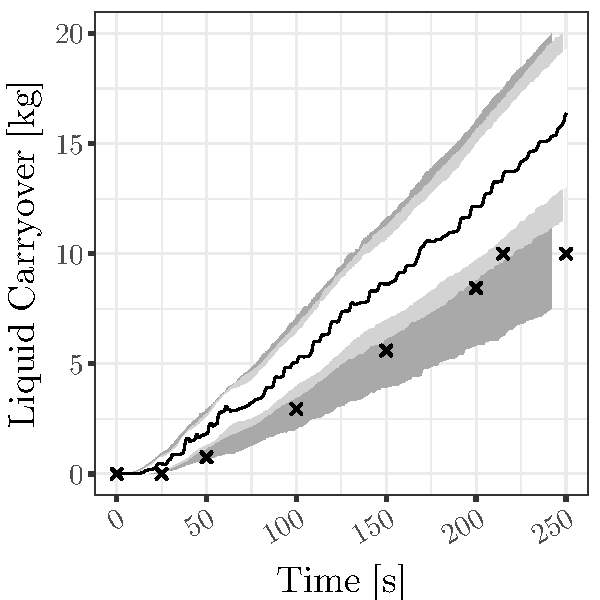
\includegraphics[width=0.5\textwidth]{../figures/chapter5/figures/plotTraceUQPosteriorAllDiscCenteredCO}
    \caption[Prior uncertainty propagation of FEBA Test No. $218$ for the pressure drop output ($DP$).]{Uncertainty propagation of the prior parameters uncertainty of \gls[hyper=false]{feba} Test No. $218$ for the pressure drop output ($TC$) at different axial segments using \gls[hyper=false]{trace}.}
    \label{fig:ch5_plot_trace_uq_posterior_alldisccentered_co}
\end{figure}

% FEBA Test No. 218 Prior Uncertainty Propagation, TC
\clearpage
\begin{sidewaysfigure}
	\centering
	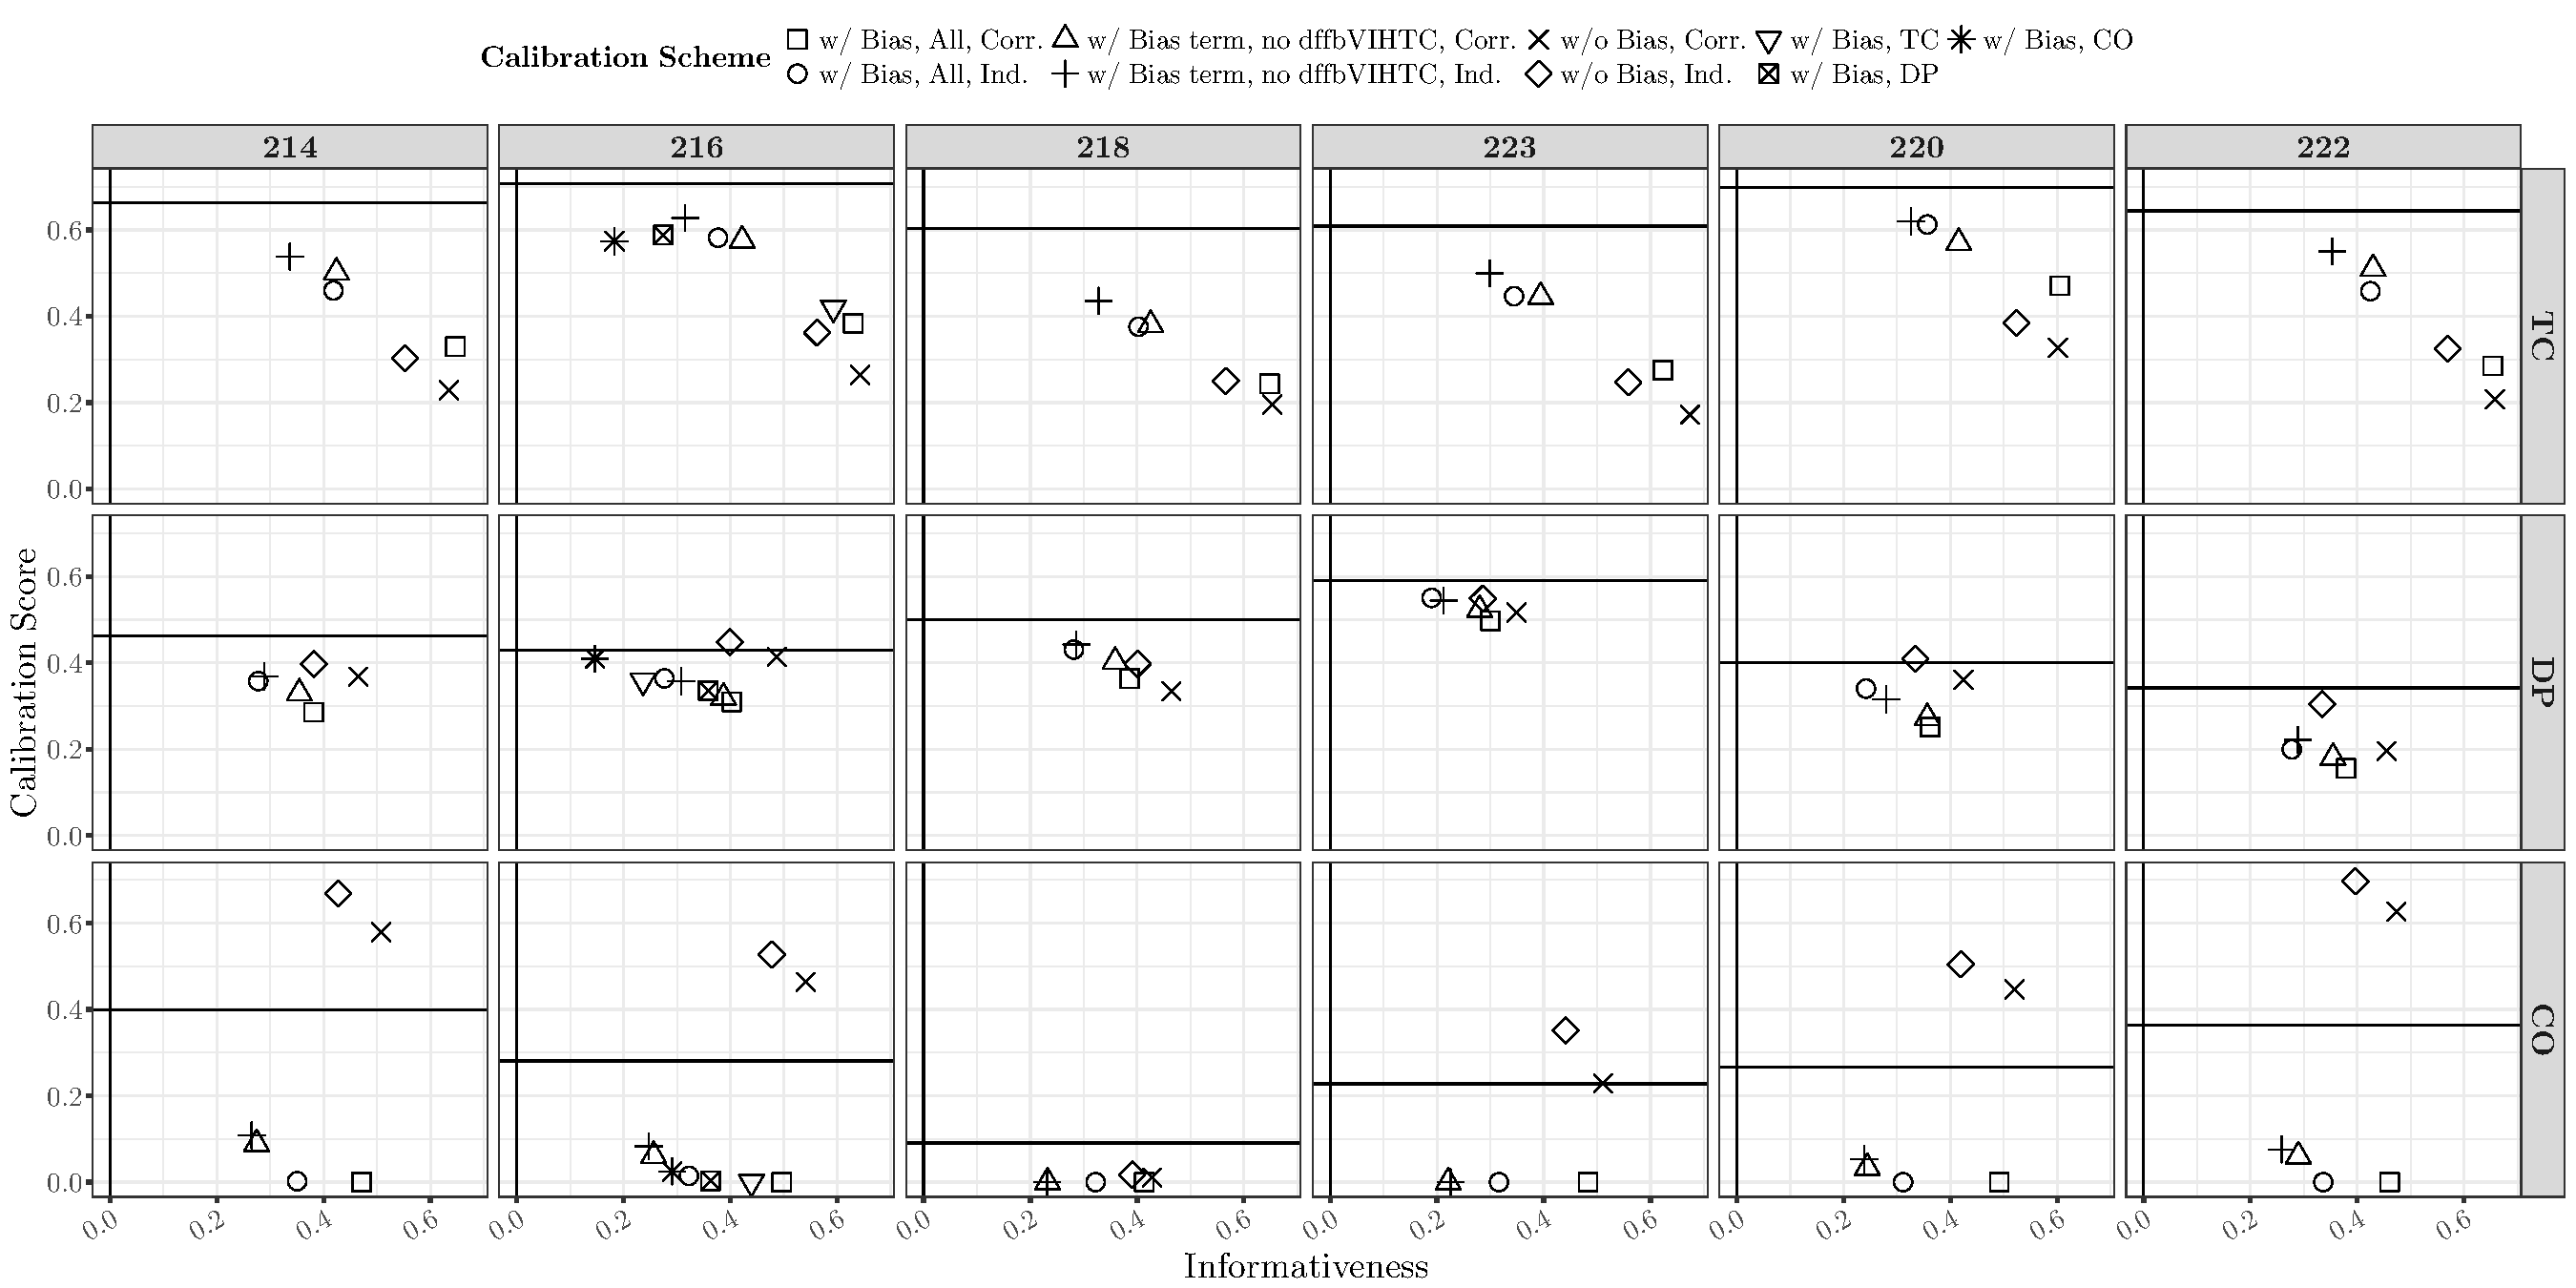
\includegraphics[width=1.0\textwidth]{../figures/chapter5/figures/plotCalibInfo}
		\captionof{figure}[Calibration score vs. Informativeness for different posterior samples propagated on all the FEBA tests.]{Calibration score vs. Informativeness for different posterior samples propagated on all the gls[hyper=false]{feba} tests. Vertical lines indicate the informativeness of the prior uncertainty (defined as $0$) while the horizontal lines indicate the initial Calibration score (i.e., that of the prior).}
	\label{fig:ch2_plot_trace_uq_prior_tc_218}
\end{sidewaysfigure}
\clearpage
